
\chapter{Statistics and Probability}
\section{Definition of Moments}
Let $x\in\mathbb R^{n}$ is a random variable.
We write $m = E[x]\in\mathbb R^n$ for the expectation and
$M=\mathrm{Var}[x] = E[(x-m)(x-m)^T]$ for the covariance (when these quantities are defined.)

In tensor diagrams, we will use square brackets:
\[
\mathbin{\begin{tikzpicture}[baseline=(n0.base), inner sep=1pt]
   \node (n0) at (0,0) {$m=[$};
   \node [right=1em of n0] (n1) {$x]$};
   \draw (n0) -- (n1);
\end{tikzpicture}}
\quad\text{and}\quad
\mathbin{\begin{tikzpicture}[baseline=(n0.base), inner sep=1pt]
   \node (n0) at (0,0) {$M=[$};
   \node [right=1em of n0] (n1) {$(x\ominus m)$};
   \node [right=.5em of n1] (n2) {$(x\ominus m)$};
   \node [right=1em of n2] (n3) {$]$};
   \draw (n0) -- (n1);
   \draw (n2) -- (n3);
\end{tikzpicture}}
\]
We will use the circled minus, $\ominus$, to distinguish the operation from contraction edges.

We can also define the third and fourth centralized moment tensors
\[
   M_3=
   \renewcommand*{\arraystretch}{1.3}
   \begin{bmatrix}
      \vecmatvec{1em}{(x\ominus m)}{}{} \\
      \vecmatvec{1em}{(x\ominus m)}{}{} \\
      \vecmatvec{1em}{(x\ominus m)}{}{}
   \end{bmatrix}
\quad\text{and}\quad
M_4=
   \renewcommand*{\arraystretch}{1.3}
   \begin{bmatrix}
      \vecmatvec{1em}{(x\ominus m)}{}{} \\
      \vecmatvec{1em}{(x\ominus m)}{}{} \\
      \vecmatvec{1em}{(x\ominus m)}{}{} \\
      \vecmatvec{1em}{(x\ominus m)}{}{}
   \end{bmatrix}
.
\]
These are less common in introductory causes, even though the scalar third and fourth moment are common.
This is presumably because they require higher order tensors.

If the entries of $x$ are independent, the non-diagonal entries disappear, so we get
\[
M =
\left[
   \begin{tikzpicture}[baseline=(c.base), inner sep=1pt]
      \node (T1) {$(x\ominus m)$};
      \node (T2)[below=.5em of T1] {$(x\ominus m)$};
      \node (c)[right=.7em of T1, yshift=-1em] {$\sbullet$};
      \draw (T1) -- (c);
      \draw (T2) -- (c);
      \draw (c) -- ++(.7em,0);
   \end{tikzpicture}
\right]
\quad\text{and}\quad
M_3 =
\left[
   \begin{tikzpicture}[baseline=(T2.base), inner sep=1pt]
      \node (T1) {$(x\ominus m)$};
      \node (T2)[below=.5em of T1] {$(x\ominus m)$};
      \node (T3)[below=.5em of T2] {$(x\ominus m)$};
      \node (c)[right=.7em of T2] {$\sbullet$};
      \draw (T1) -- (c);
      \draw (T2) -- (c);
      \draw (T3) -- (c);
      \draw (c) -- ++(.7em,0);
   \end{tikzpicture}
\right]
\quad\text{and so on.}
\]
If the entries are also identically distributed, we simply have
\[
   M = \sigma^2
   \,
\begin{tikzpicture}[baseline=(T.base), inner sep=0]
   \node (T) {$\sbullet$};
   \draw (T) -- ++(0,.3);
   \draw (T) -- ++(0,-.3);
\end{tikzpicture}
   \text{ and }
   M_3 = \mathrm{E}[(x_0-m_0)^3]
\begin{tikzpicture}[baseline=(T.base), inner sep=0]
   \node (T) {$\sbullet$};
   \draw (T) -- ++(0,.3);
   \draw (T) -- ++(-.2,-.3);
   \draw (T) -- ++(.2,-.3);
\end{tikzpicture}
.
\]

\section{Expectation of Linear Combinations}
General principle: The ``linearity of expectation'' lets you pull out all parts of the graph not involving $X$.
\[
   \vcenter{\hbox{
      \import{figures/}{linearityOfExpectation.pdf_tex}
   }}
\]
where $M_3$ is the expectation
\(
\left[
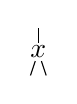
\begin{tikzpicture}[baseline=(T.base), inner sep=1pt]
   \node (T) {$x$};
   \draw (T) -- ++(0,.3);
   \draw (T) -- ++(-.1,-.3);
   \draw (T) -- ++(.1,-.3);
\end{tikzpicture}
\,
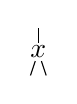
\begin{tikzpicture}[baseline=(T.base), inner sep=1pt]
   \node (T) {$x$};
   \draw (T) -- ++(0,.3);
   \draw (T) -- ++(-.1,-.3);
   \draw (T) -- ++(.1,-.3);
\end{tikzpicture}
\,
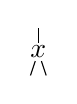
\begin{tikzpicture}[baseline=(T.base), inner sep=1pt]
   \node (T) {$x$};
   \draw (T) -- ++(0,.3);
   \draw (T) -- ++(-.1,-.3);
   \draw (T) -- ++(.1,-.3);
\end{tikzpicture}
\right]
\),
which is an order-9 tensor with no dependence on the constants $A$, $B$, $C$ and $D$.
In practice you would want to name the edges to keep track of what gets multiplied with what.

\subsection{Linear Forms}
The Matrix Cookbook gives the following simple expectations:
\begin{align*}
   \tag{312}
   \E[AXB+C] &= A \E[X] B + C
   &
   \renewcommand*{\arraystretch}{1.3}
   \begin{bmatrix}
      \matmul{A,X,B} \\+\, \matmul{C}
   \end{bmatrix}
   &=
   \renewcommand*{\arraystretch}{1.3}
   \begin{matrix}
      \matmul{A,[X],B} \\+\, \matmul{C}
   \end{matrix}
   %%%%%%%%%%%%%%%%%%%%%%%%%%%%%%%%%%%%%%%%
   \\
   \tag{313}
   \mathrm{Var}[Ax] &= A \mathrm{Var}[x] A^T
   &
   \renewcommand*{\arraystretch}{1.3}
   \begin{bmatrix}
      \vecmatvec{.5em}{A}{}{x} \ominus [\vecmatvec{.5em}{A}{}{x}] \\
      \vecmatvec{.5em}{A}{}{x} \ominus [\vecmatvec{.5em}{A}{}{x}]
   \end{bmatrix}
   &=
   \renewcommand*{\arraystretch}{1.3}
   \begin{bmatrix}
      \vecmatvec{.5em}{A}{}{(x\ominus m)} \\
      \vecmatvec{.5em}{A}{}{(x\ominus m)}
   \end{bmatrix}
 \\&&&=
   \vcenter{\hbox{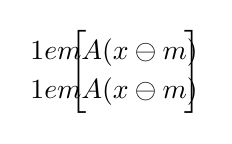
\begin{tikzpicture}[inner sep=1pt]
      \node (n1) at (0,-.25) {$\vecmatvec{1em}{A}{}{(x\ominus m)}$};
      \node (n2) at (0,.25) {$\vecmatvec{1em}{A}{}{(x\ominus m)}$};
      \node at (-.45, 0) {$\Bigg[$};
      \node at (1, 0) {$\Bigg]$};
   \end{tikzpicture}}}
 \\&&& =
   \vecmatvec{.5em}{}{A,M_2,A}{}
\end{align*}

\subsection{Quadratic Forms}
We often prefer to write expectations in terms of the simple centered moments, which we can do by pulling out the mean:
\renewcommand*{\arraystretch}{1}
\[
\begin{bmatrix}
   x - \\
   x -
\end{bmatrix}
=
\begin{bmatrix}
   (x\ominus m) - \\
   (x\ominus m) -
\end{bmatrix}
+
\begin{array}{c}
   m - \\
   m -
\end{array}
\]
This makes it easy to handle the quadratic forms from the Matrix Cookbook:
\renewcommand*{\arraystretch}{1}
\begin{align*}
   \E[x^T A x]
   &= \mathrm{Tr}(A \Sigma) + m^T A m
   &
   [\vecmatvec{.5em}{x}{A}{x}]
   &=
   \left(
      \begin{bmatrix}
         (x\ominus m) - \\
         (x\ominus m) -
      \end{bmatrix}
      +
      \begin{array}{c}
         m - \\
         m -
      \end{array}
   \right)
   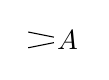
\begin{tikzpicture}[baseline=(A.base), inner sep=1pt]
      \node (A) {$A$};
      \draw (A) -- ++(-.5, .1);
      \draw (A) -- ++(-.5, -.1);
   \end{tikzpicture}
   \\
   &&&=
   \mathbin{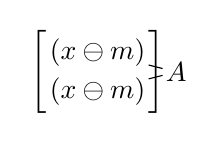
\begin{tikzpicture}[baseline=(A.base), inner sep=1pt]
      \node (n1) at (0,-.25) {$(x\ominus m)$};
      \node (n2) at (0,.25) {$(x\ominus m)$};
      \node at (-.75, 0) {$\Bigg[$};
      \node at (.75, 0) {$\Bigg]$};
      \node (A) at (1, 0) {$A$};
      \draw (n1) -- (A);
      \draw (n2) -- (A);
   \end{tikzpicture}}
   +
   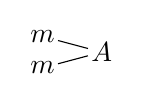
\begin{tikzpicture}[baseline=(A.base), inner sep=1pt]
      \node (A) {$A$};
      \node (m1) at (-.75, .2) {$m$};
      \node (m2) at (-.75, -.2) {$m$};
      \draw (m1) -- (A) -- (m2);
   \end{tikzpicture}
   \\
   &&&=
   \trace{\Sigma,A}2
   +
   \vecmatvec{.5em}{m}{A}{m}
   \\
   E[\mathbf{x}^T A\mathbf{x}] &= \text{Tr}(AM) + m^T Am \tag{318} \\
\end{align*}
Note, the later is really a quartic form.

Also, assume $\mathbf{x}$ to be a stochastic vector with mean m, and covariance M.
Then
\begin{align*}
   \text{Var}[\mathbf{x}^T A\mathbf{x}] &= 2\mu_2^2\text{Tr}(A^2) + 4\mu_2 c^T A^2 c + 4\mu_3 c^T Aa + (\mu_4 - 3\mu_2^2)a^T a \tag{319} \\
   E[(A\mathbf{x} + a)(B\mathbf{x} + b)^T] &= AMB^T + (Am + a)(Bm + b)^T \tag{320} \\
   E[\mathbf{x}\mathbf{x}^T] &= M + mm^T \tag{321} \\
   E[\mathbf{x} a^T \mathbf{x}] &= (M + mm^T)a \tag{322} \\
   E[\mathbf{x}^T a\mathbf{x}^T] &= a^T(M + mm^T) \tag{323} \\
   E[(A\mathbf{x})(A\mathbf{x})^T] &= A(M + mm^T)A^T \tag{324} \\
   E[(\mathbf{x} + a)(\mathbf{x} + a)^T] &= M + (m + a)(m + a)^T \tag{325} \\
   E[(A\mathbf{x} + a)^T(B\mathbf{x} + b)] &= \text{Tr}(AMB^T) + (Am + a)^T(Bm + b) \tag{326} \\
   E[\mathbf{x}^T \mathbf{x}] &= \text{Tr}(M) + m^T m \tag{327} \\
   E[\mathbf{x}^T A\mathbf{x}] &= \text{Tr}(AM) + m^T Am \tag{328} \\
   E[(A\mathbf{x})^T(A\mathbf{x})] &= \text{Tr}(AMA^T) + (Am)^T(Am) \tag{329} \\
   E[(\mathbf{x} + a)^T(\mathbf{x} + a)] &= \text{Tr}(M) + (m + a)^T(m + a) \tag{330}
\end{align*}

\begin{walign}
   \tag{319}
   \text{Var}[x^T A x] &= 2\mu_2^2\text{Tr}(A^2) + 4\mu_2 c^T A^2 c + 4\mu_3 c^T A a + (\mu_4 - 3\mu_2^2)a^T a
   &&
   \begin{tikzpicture}[baseline=(a0.base), inner sep=1pt]
      % Start with y = x^T A x
      \node (a0) {$x^T A x$};
      \node[right=1em of a0] (sq) {${}^2$};
      \draw[d] (sq.east) -- ++(.2,.2);
      \draw[d] (sq.east) -- ++(.3,.1);
   \end{tikzpicture}
 \\&&&=
   \begin{tikzpicture}[baseline=(A.base), inner sep=1pt]
      % Expand x into m + (x⊖m)
      \node (x1) {$(x \ominus m)$};
      \node[right=1em of x1] (A) {$A$};
      \node[right=1em of A] (x2) {$(x \ominus m)$};
      \draw (x1) -- (A) -- (x2);
      \node[above=0.3em of A] {$+$ terms\,with\,m$\,\,$};
      % This diagram represents one of the central terms of the quartic expansion
   \end{tikzpicture}
   +
   \dots
 \\&&&=
   % Here we would show all pairings using Isserlis/Wick expansions:
   % Terms with (x⊖m)⁴ → μ_4 or μ_2²
   % Terms with (x⊖m)³ m → μ_3
   % Terms with (x⊖m)² m² → μ_2
   % Terms with m³ (x⊖m) → linear terms in μ_3
   % and pure m^4 terms
   % After careful collection of all terms:
   \begin{tikzpicture}[baseline=(a0.base), inner sep=1pt]
      \node (res) {$2\mu_2^2\text{Tr}(A^2) + 4\mu_2 c^T A^2 c + 4\mu_3 c^T A a + (\mu_4 - 3\mu_2^2)a^T a$};
   \end{tikzpicture}
\end{walign}

\begin{walign}
   \tag{320}
   E[(A x + a)(B x + b)^T] &= A M B^T + (A m + a)(B m + b)^T
   &&
   \begin{tikzpicture}[baseline=(A.base), inner sep=1pt]
      \node (A) {$A$};
      \node[right=.5em of A] (x) {$x$};
      \node[right=.7em of x] (+a) {$+\,a$};
      \node[right=2em of +a] (B) {$B$};
      \node[right=.5em of B] (x2) {$x$};
      \node[right=.7em of x2] (+b) {$+\,b$};
      \draw[d] (+b.east) -- ++(.2,.2);
      \draw[d] (+b.east) -- ++(.3,.1);
   \end{tikzpicture}
 \\&&&=
   \begin{tikzpicture}[baseline=(A.base), inner sep=1pt]
      % Distribute expectation:
      % E[(A x)(B x)^T] + E[(A x)b^T] + E[a(B x)^T] + a b^T
      \node (A) {$A$};
      \node[right=.5em of A] (xx) {$[x x^T]$};
      \node[right=.5em of xx] (B) {$B^T$};
      \draw (A) -- (xx) -- (B);
      \draw[d] (B.east) -- ++(.2,-.2);
      \draw[d] (B.east) -- ++(.3,-.1);
   \end{tikzpicture}
   +
   \begin{tikzpicture}[baseline=(m.base), inner sep=1pt]
      \node (A) {$A$};
      \node[right=.5em of A] (m) {$m$};
      \node[right=.5em of m] (b) {$b^T$};
      \draw (A) -- (m);
      \draw (m) -- (b);
   \end{tikzpicture}
   +
   \begin{tikzpicture}[baseline=(a.base), inner sep=1pt]
      \node (a) {$a$};
      \node[right=.5em of a] (B) {$B$};
      \node[right=.5em of B] (m2) {$m^T$};
      \draw (a) -- (B);
      \draw (B) -- (m2);
   \end{tikzpicture}
   +
   \begin{tikzpicture}[baseline=(a.base), inner sep=1pt]
      \node (a) {$a$};
      \node[right=.5em of a] (b) {$b^T$};
      \draw (a) -- (b);
   \end{tikzpicture}
 \\&&&=
   A(M + m m^T) B^T + (A m + a)(B m + b)^T
   \quad=\quad A M B^T + (A m + a)(B m + b)^T.
\end{walign}

\subsection{Cubic Forms}
When $x$ is a stochastic vector with mean vector $m$,
it can be convenient to expand the raw third moment in terms of the central moments:
\renewcommand*{\arraystretch}{1}
\begin{align*}
\begin{bmatrix}
   x - \\
   x - \\
   x -
\end{bmatrix}
&=
\begin{bmatrix}
   (x\ominus m) - \\
   (x\ominus m) - \\
   (x\ominus m) -
\end{bmatrix}
\vspace{-.5em}
+
3
\hspace{-.25em}
\begin{array}{l}
\begin{bmatrix}
   (x\ominus m) -
\end{bmatrix}\\[.1em]
\begin{bmatrix}
   m - \\
   m -
\end{bmatrix}
\end{array}
\hspace{-.5em}
+
3
\hspace{-.25em}
\begin{array}{l}
\begin{bmatrix}
   m -
\end{bmatrix}\\[.1em]
\begin{bmatrix}
   (x\ominus m) - \\
   (x\ominus m) -
\end{bmatrix}
\end{array}
\hspace{-.5em}
+
\hspace{-.5em}
\begin{array}{c}
\begin{bmatrix}
   m -
\end{bmatrix}\\[.1em]
\begin{bmatrix}
   m -
\end{bmatrix}\\[.1em]
\begin{bmatrix}
   m -
\end{bmatrix}
\end{array}
%
\\&=
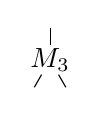
\begin{tikzpicture}[baseline=(T.base), inner sep=1pt]
   \node (T) {$M_3$};
   \draw (T) -- ++(0,.4);
   \draw (T) -- ++(-.2,-.35);
   \draw (T) -- ++(.2,-.35);
\end{tikzpicture}
+
3
\hspace{-.25em}
\begin{array}{c}
   m - \\
   -M-
\end{array}
\hspace{-.5em}
+
\begin{array}{c}
   m - \\
   m - \\
   m -
\end{array}
\end{align*}
TODO: The edges from the $m,M$ term needs to be symmetrized.

Assume \(\mathbf{x}\) to be a stochastic vector with independent coordinates, mean \(m\),
covariance \(M\) and central moments \(v_3 = \mathbb{E}[(\mathbf{x} - m)^3]\). Then (see [7])
\begin{align*}
&\mathbb{E}[(A\mathbf{x} + a)(B\mathbf{x} + b)^T (C\mathbf{x} + c)]
\\&\quad=
A\,\mathrm{diag}(B^T C) v_3
\\&\quad+
(Am + a) \mathrm{Tr}(BMC^T)
\\&\quad+
AMC^T (Bm + b)
\\&\quad\,+
AMB^T (Cm + c)
\\&\quad+
(Am + a)(Bm + b)^T (Cm + c)
\\
  &\mathbb{E}[\mathbf{x} \mathbf{x}^T \mathbf{x}]
\\&\quad=
   v_3
\\&\quad+
   2 Mm
\\&\quad+
   (\text{Tr}(M) + m^T m) m
\end{align*}





\section{Weighted Scalar Variable}
Let $y=w^T x$, and let $m=E[y]$, then
\begin{align*}
   \E[y] &= m = w^T \mu
   \\
   \E[(y\ominus m)^2] &= \vecmatvec{.5em}{w}{M_2}{w}
   \\
   \E[(y\ominus m)^3] &=
   \mathbin{\begin{tikzpicture}[baseline=(a0.base), inner sep=1pt]
      \node (a0) {$M_3$};
      \node[above=.3em of a0] (n0) {$w$};
      \node[right=.3em of a0] (n1) {$w$};
      \node[left=.3em of a0] (n3) {$w$};
      \draw (a0.north) -- (n0);
      \draw (a0.east) -- (n1);
      \draw (a0.west) -- (n3);
   \end{tikzpicture}}
   \\
   \E[(y\ominus m)^4] &=
   \mathbin{\begin{tikzpicture}[baseline=(a0.base), inner sep=1pt]
      \node (a0) {$M_4$};
      \node[above=.3em of a0] (n0) {$w$};
      \node[right=.3em of a0] (n1) {$w$};
      \node[below=.3em of a0] (n2) {$w$};
      \node[left=.3em of a0] (n3) {$w$};
      \draw (a0.north) -- (n0);
      \draw (a0.east) -- (n1);
      \draw (a0.south) -- (n2);
      \draw (a0.west) -- (n3);
   \end{tikzpicture}}
\end{align*}
For specific distributions, like $x$ Gaussian, we can often reduce the moment tensors further.
Khintchine's inequality also gives a way to bound all of these in terms of $E[(y-m)^2]$.


Similarly,
\[
\mathbb{E}[(y\ominus m_y)^3]
=
\begin{tikzpicture}[baseline=(M3.base), inner sep=1pt]
   \node (M3) {$M_3$};
   \node[above=.3em of M3] (w0) {$w$};
   \node[left=.3em of M3] (w1) {$w$};
   \node[right=.3em of M3] (w2) {$w$};
   \draw (M3) -- (w0);
   \draw (M3) -- (w1);
   \draw (M3) -- (w2);
\end{tikzpicture}
= w^T M_3 (w,w).
\]
\section{Gaussian Moments}

For a Gaussian vector $x \sim \mathcal{N}(m,M)$:
- All odd centered moments vanish: $M_3 = 0$, etc.
- Even moments can be computed via Isserlis' theorem.

For instance:
\[
\mathbb{E}[(x \ominus m)^{\otimes 4}]
=
M \otimes M + M \otimes M + \dots
\]
(summing over the different pairings of indices).

\subsection{Gaussian Integration by Parts}
If $X$ is a tensor with Gaussian entries, zero mean, and some covariance,
% General principle for Gaussian expectations.
Stein's lemma gives the following very general equation, for any differentiable function $f$:
\[
   \vcenter{\hbox{
      \import{figures/}{steins.pdf_tex}
   }}
\]
Combined with the tensor chain rule from chapter~\ref{chapter:functions}, this can be a very powerful way to evaluate many hard expectations.

\subsection{Mean and covariance of linear forms}
TODO
\subsection{Mean and variance of square forms}
TODO
\subsection{Cubic forms}
TODO
\subsection{Mean of Quartic Forms}
TODO
For the fourth moment of a Gaussian with zero mean, Isserlis' theorem gives:
\[
E[x_i x_j x_k x_l] = M_{ij}M_{kl} + M_{ik}M_{jl} + M_{il}M_{jk}.
\]
With a nonzero mean, add corresponding terms involving $m$.

\subsection{Mixture of Gaussians}
For a mixture of Gaussians:
\[
   x \sim \sum_k \pi_k \mathcal{N}(m_k, M_k),
\]
the moments are weighted sums:
\[
   E[x] = \sum_k \pi_k m_k, \quad
   \mathrm{Var}[x] = \sum_k \pi_k (M_k + m_k m_k^T) - \left(\sum_k \pi_k m_k\right)\left(\sum_k \pi_k m_k\right)^T.
\]
Higher moments similarly combine via linearity.

\subsection{Derivatives}
Derivatives of moments with respect to $m$ or $M$ can be found by differentiating under the integral sign, and using Stein's lemma for Gaussian cases.

\section{Exercises}
\begin{exercise}
   \begin{align*}
   \mathbb{E}[(A\mathbf{x} + a)(A\mathbf{x} + a)^T (A\mathbf{x} + a)] = 
   \text{Adiag}(A^T A) v_3 \\
   + [2 AMA^T + (A\mathbf{x} + a)(A\mathbf{x} + a)^T] (Am + a) \\
   + \text{Tr}(AMA^T)(Am + a)
   \end{align*}

   \begin{align*}
   \mathbb{E}[(A\mathbf{x} + a) b^T (C\mathbf{x} + c)(D\mathbf{x} + d)^T] = 
   (A\mathbf{x} + a) b^T (CMD^T + (Cm + c)(Dm + d)^T) \\
   + (AMC^T + (Am + a)(Cm + c)^T) b(Dm + d)^T \\
   + b^T (Cm + c)(AMD^T - (Am + a)(Dm + d)^T)
   \end{align*}
\end{exercise}
\begin{exercise}
   Find more identities in the \href{http://www.ee.ic.ac.uk/hp/staff/dmb/matrix/expect.html}{Matrix Reference Manual} and try to prove them.
   Also try to verify your derivations using tensorgrad.
\end{exercise}
